\documentclass[12pt, letterpaper]{article}
\usepackage{graphicx}
\graphicspath{{images/}}
\usepackage{amsmath}
\usepackage{float}
\usepackage{url}
\usepackage{subcaption}
\setlength{\parindent}{0pt}
\setlength{\parskip}{1em}
\title{Project 3: The Ising Model}
\author{Max Halpern and Ben Schuster}
\date{5/6/26}
\begin{document}
\maketitle

\begin{itemize}
	\item Extend Mean-field Approximation discussion
	\begin{itemize}
		\item i dont know what this means
	\end{itemize}
	\item Monte Carlo Simulation
	\begin{itemize}
		\item Correlation Functions and their behavior near phase transition (Max) (Problem 8.29) \textbf{(DONE)}
		\item Block-spin Transformation and Renormalization (Ben) (Problem 8.32)
	\end{itemize}
\end{itemize}

Different geometries? - could be hard to implement in existing code

Next nearest neighbors?

External B \textbf{(DONE unless you want to add something)}

\textbf{Problem 8.29}

To quantify the clustering of alignments within an Ising magnet, we define a quantity called the \textbf{correlation function}, $c(r)$. Take any two dipoles, $i$ and $j$, separated by a distance $r$, and compute the product of their states: $s_i s_j$. This product is 1 if the dipoles are parallel and -1 if the dipoles are antiparallel. Now average this quantity over \textit{all} pairs that are separated by a fixed distance $r$, to obtain a measure of the tendency of dipoles to be "correlated" over this distance. Finally, to remove the effect of any overall magnetization of the system, subtract off the square of the average $s$. Written as an equation, then, the correlation function is

\begin{equation*}
	c(r) = \overline{s_i s_j} - \overline{s_i}^2
\end{equation*}

where it is understood that the first term averages over all pairs at the fixed distance $r$. Technically, the averages should also be taken over all possible states of the system, but don't do this yet. 

\textbf{(a)} Add a routine to the \texttt{ising} program to compute the correlation function for the current state of the lattice, averaging over all pairs separated either vertically or horizontally (but not diagonally) by $r$ units of distance, where $r$ varies from 1 to half the lattice size. Have the program execute this routine periodically and plot the results as a bar graph.

\textbf{Answer:} I ran the correlation for a lattice of size 100 after one simulation and created the following bar graph:

\begin{figure}[H]
	\centering
	
\includegraphics[scale=0.75]{corrA.png}
\end{figure}

We can see the function decays exponentially as $r$ increases and after around $r=20$ it is roughly zero.

\textbf{(b)} Run this program at a variety of temperatures above, below, and near the critical point. Use a lattice size of at least 20, preferably larger (especially near the critical point). Describe the behavior of the correlation function at each temperature.

\textbf{Answer:} I created charts of the correlation for the following temperatures: 0.5, 1, 2, 2.27 (the critical temperature), 3, and 5:

\begin{figure}[H]
	\centering
	
	\begin{subfigure}{0.32\linewidth}
		
\includegraphics[width=\linewidth]{corrB_0.5.png}
	\end{subfigure}
	\hfill
	\begin{subfigure}{0.32\linewidth}
		
\includegraphics[width=\linewidth]{corrB_1.png}
	\end{subfigure}
	\hfill
	\begin{subfigure}{0.32\linewidth}
		
\includegraphics[width=\linewidth]{corrB_2.png}
	\end{subfigure}
	
	\vspace{0.5em}
	
	\begin{subfigure}{0.32\linewidth}
		
\includegraphics[width=\linewidth]{corrB_Tc.png}
	\end{subfigure}
	\hfill
	\begin{subfigure}{0.32\linewidth}
		
\includegraphics[width=\linewidth]{corrB_3.png}
	\end{subfigure}
	\hfill
	\begin{subfigure}{0.32\linewidth}
		
\includegraphics[width=\linewidth]{corrB_5.png}
	\end{subfigure}
\end{figure}

We can see that as temperature increases, the correlation function drops off much more rapidly with increasing $r$. At temperatures below $T_c$, there is significant correlation at large distances, which makes sense because this is the regime in which large scale structures appear. Above $T_c$, the correlation function drops to 0 rapidly because there are at most small structures, and the magnetization as a whole is largely uncorrelated.

\textbf{(c)} Now add code to compute the \textit{average} correlation function over the duration of a run. (However, it's best to let the system "equilibrate" to a typical state before you begin accumulating averages.) The \textbf{correlation length} as defined as the distance over which the correlation function decreases by a factor of $e$. Estimate the correlation length at each temperature, and plot a graph of the correlation length vs. \texttt{T}.

\textbf{Answer:} By converting to a scatter plot and log scale, I can come up with a linear fit to estimate the correlation length, which should be the negative reciprocal of the slope:

\begin{figure}[H]
	\centering
	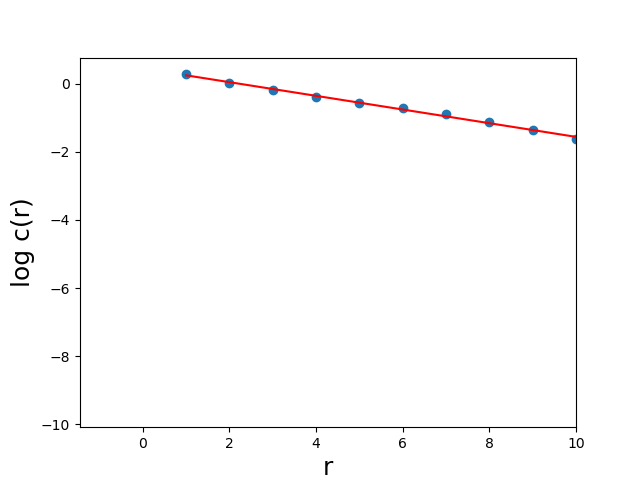
\includegraphics[scale=0.75]{corrC_1.png}
\end{figure}

I was able to plot correlation lengths for a series of temperatures, including the critical temperature:

\begin{figure}[H]
	\centering
	
\includegraphics[scale=0.75]{corrC_2.png}
\end{figure}

It can be seen that the correlation length generally decreases with $T$. Past the critical temperature, the correlation length seems to bottom out between 2-4. This is telling us that below $T_c$,  there is correlation across a relatively long distance, suggesting large structures. Above $T_c$, what correlation exists is only on short scales, implying small structures.

\textbf{Applying an External Field}

If an external magnetic field is applied to our lattice, it tacks on another term to our energy:

\begin{equation*}
	U = -\epsilon\sum_{i,j\ pairs} s_i s_j - B \sum_{i} s_i
\end{equation*}

In the Metropolis algorithm, this makes the state aligned with the magnetic field much more likely. This is reflected in the correlation function among other things. Consider the example of $T=2.27$ now with a magnetic field $B=0.05$:

\begin{figure}[H]
	\centering
	
\includegraphics[scale=0.75]{extB_1.png}
\end{figure}

In this case the lattice converged almost completely to a unified magnetization, and the correlation function also converges to just over 0.5. This means that over any length scale we have correlation, because almost the entire lattice is pointed in one direction. If we plot correlation lengths for many temperatures values with $B=0.05$:

\begin{figure}[H]
	\centering
	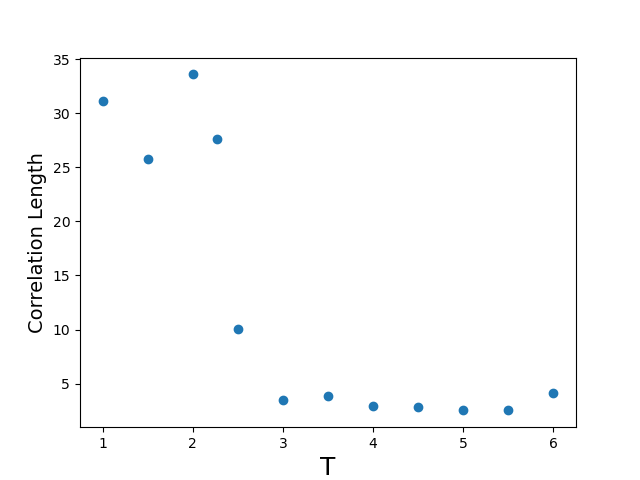
\includegraphics[scale=0.75]{extB_2.png}
\end{figure}

Interestingly, the critical temperature still appears to be at $T_c  =2.27$. The length in absolute terms increases in absolute terms below $T_c$ but the dropoff occurs in the same place and above $T_c$ the length again hovers between 2-4. 

\end{document}
